
%%%% CAPÍTULO 1 - INTRODUÇÃO
%%
%% Deve apresentar uma visão global da pesquisa, 
%% incluindo: breve histórico, importância e
%% justificativa da escolha do tema, delimitações
%% do assunto, formulação de hipóteses e objetivos
%% da pesquisa e estrutura do trabalho.

% Perguntas que podem guiar a introdução - não necessariamente irá ter a resposta para tudo, isso depende da área.
% 1 - Qual é o contexto em que seu trabalho está inserido?
% 2 - Qual é o problema que motiva a existência deste trabalho?
% 3 - Qual é a visão geral da literatura sobre o problema e como é tratado
% 4 - Por que a solução na literatura não é o suficiente para ?
% 5 - Como seu trabalho trata o problema ?
% 6 - como seu trabalho foi avaliado para comprovar que tratou adequadamente o problema?
% 7 - De forma geral quais foram os resultados ?
% 8 - Quais foram as contribuições do seu trabalho?
% 9 -  Como o restante da Dissertação ou Tese está organizada ?


\chapter{Introdução}
\label{cap:introducao}

As inundações em áreas urbanas apresentam riscos significativos à infraestrutura, saúde pública e meio ambiente. A água inundada pode levar a muitos problemas, incluindo a interrupção de transportes e serviços essenciais (energia elétrica, internet, etc.) . 
Para os órgãos governamentais responsáveis pelo monitoramento de áreas urbanas, como o \acrfull{cor}, a observação constante dessas áreas urbanas é crucial para a emissão de alertas precoces e respostas eficazes. 
A detecção e avaliação oportuna dos riscos de inundação permitem que as autoridades implementem planos de evacuação, desloquem serviços de emergência e iniciem medidas de controle de inundação para minimizar danos e proteger vidas.

O monitoramento pelo \acrshort{cor} é realizado na própria sala de controle, onde dezenas de funcionários monitoram uma quantidade ainda maior de telas que exibem as milhares de câmeras da cidade do Rio de Janeiro, como pode ser visto na Figura \ref{fig:cor}, tornando isto um trabalho árduo.

\section{Objetivos}

O monitoramento atualmente realizado pelo \acrshort{cor} não é automatizado. Este monitoramento não só é dependente da mão-de-obra dos funcionários frente a diversas telas, como também depende em parte de notificações enviadas por terceiros, utilizando o aplicativo do \acrshort{cor} para reportar problemas na cidade de forma direta.

\begin{figure}[htb]
\centerline{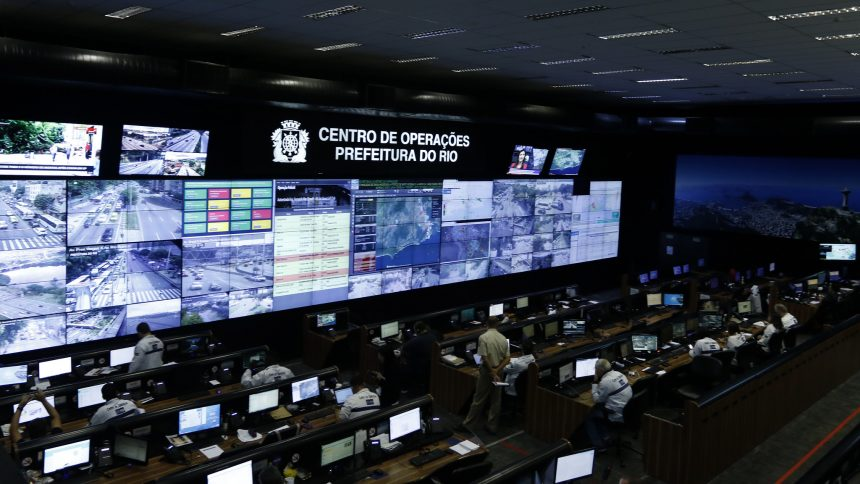
\includegraphics[width=0.9\linewidth]{images/46627458084_451cf87027_k.jpg}}
\caption{Sala central do Centro de Operações do Rio}
\label{fig:cor}
\end{figure}

Com base em diversas pesquisas sobre o problema das inundações urbanas utilizando diferentes Redes Neurais Convolucionais (CNN, do inglês \acrlong{cnn}),
apresentadas na Seção \ref{sec:trabalhos_alagamento}, 
a presente dissertação visa desenvolver uma abordagem inicial utilizando \acrshort{cnn}s com aprendizado por transferência (\textit{transfer learning}), treinadas em um conjunto de dados original, 
para não apenas facilitar o monitoramento das milhares de câmeras na cidade do Rio de Janeiro pelo \acrshort{cor}, 
mas também notificar automaticamente quando uma rua estiver em uma situação que necessite de ação do \acrshort{cor}.

Para automatizar o monitoramento da situação de alagamento da cidade do Rio de Janeiro, cinco arquiteturas de redes neurais foram treinadas e avaliadas. Todos os modelos foram treinados em conjunto de dados original formado por imagens do circuito de câmeras do Centro de Operações do Rio.
Todas as câmeras neste conjunto de dados são fixas, de forma que não há nenhuma modificação na paisagem ao longo do dia.

\section{Organização do Texto}\label{Organização do texto}

O capítulo \ref{cap:fundamentação} explica brevemente os conceitos mais importantes para o desenvolvimento deste trabalho, começando por técnicas de processamento de imagem e finalizando na abordagem dos fundamentos de redes neurais.

O capítulo \ref{cap:trabalhos} considera alguns trabalhos relevantes para o problema de classificação do estado de alagamento em regiões urbanas nos últimos 5 anos. 
Ao final, algumas características das tecnologias utilizadas em cada artigo, assim como as deste trabalho, são comparadas em uma tabela.

O capítulo \ref{cap:metodologia} descreve a metodologia usada na execução deste trabalho. 
Explicando a criação do conjunto de dados, a escolha das arquiteturas de \acrshort{cnn}s inicialmente empregadas e as métricas utilizadas para a comparação dos resultados.

O capítulo \ref{cap:resultados} apresenta e discute os resultados do treinamento das diferentes arquiteturas comparadas. 
O modelo com melhor performance é mais detalhadamente avaliado após a inclusão de alterações no pré-processamento e uso de diferentes conjuntos de dados de entrada.

O capítulo \ref{cap:conclusoes} sumariza as contribuições e limitações deste trabalho, apresentando conclusões relacionadas aos seus resultados. 
Também Discute possíveis pontos para melhoria futuras em prosseguimentos da linha de pesquisa .